 \let\negmedspace\undefined
\let\negthickspace\undefined
\documentclass[journal]{IEEEtran}
\usepackage[a5paper, margin=10mm, onecolumn]{geometry}
%\usepackage{lmodern} % Ensure lmodern is loaded for pdflatex
\usepackage{tfrupee} % Include tfrupee package

\setlength{\headheight}{1cm} % Set the height of the header box
\setlength{\headsep}{0mm}     % Set the distance between the header box and the top of the text
\usepackage{gvv-book}
\usepackage{gvv}
\usepackage{cite}
\usepackage{amsmath,amssymb,amsfonts,amsthm}
\usepackage{algorithmic}
\usepackage{graphicx}
\usepackage{textcomp}
\usepackage{xcolor}
\usepackage{txfonts}
\usepackage{listings}
\usepackage{enumitem}
\usepackage{mathtools}
\usepackage{gensymb}
\usepackage{comment}
\usepackage[breaklinks=true]{hyperref}
\usepackage{tkz-euclide} 
\usepackage{listings}
% \usepackage{gvv}                                        
\def\inputGnumericTable{}                                 
\usepackage[latin1]{inputenc}                                
\usepackage{color}                                            
\usepackage{array}                                            
\usepackage{longtable}                                       
\usepackage{calc}                                             
\usepackage{multirow}                                         
\usepackage{hhline}                                           
\usepackage{ifthen}                                           
\usepackage{lscape}



\usepackage{amsmath,amssymb}
\usepackage{booktabs}
\usepackage{tikz}
\usetikzlibrary{arrows.meta,angles,quotes}





\begin{document}

\bibliographystyle{IEEEtran}
\vspace{3cm}

\title{4.13.90}
\author{AI25BTECH11021 - Abhiram Reddy N}
% \maketitle
% \newpage
% \bigskip
{\let\newpage\relax\maketitle}

\renewcommand{\thefigure}{\theenumi}
\renewcommand{\thetable}{\theenumi}
\setlength{\intextsep}{10pt} % Space between text and floats


\numberwithin{equation}{enumi}
\numberwithin{figure}{enumi}
\renewcommand{\thetable}{\theenumi}


\section*{Question}
If the distance of the point \( \mathbf{P}(1, -2, 1) \) from the plane 
\[
x + 2y - 2z = \alpha, \quad \text{where } \alpha > 0,
\]
is 5, then the foot of the perpendicular from \( \mathbf{P} \) to the plane is:

\begin{multicols}{4}
\begin{enumerate}
    \item \( \left( \frac{8}{3}, \frac{4}{3}, -\frac{7}{3} \right) \)
    \item \( \left( \frac{4}{3}, -\frac{4}{3}, \frac{1}{3} \right) \)
    \item \( \left( \frac{1}{3}, \frac{2}{3}, \frac{10}{3} \right) \)
    \item \( \left( \frac{2}{3}, -\frac{1}{3}, \frac{5}{2} \right) \)
\end{enumerate}
\end{multicols}

\section*{Solution}

\subsection*{Step 1: Let the plane be \( \mathbf{n}^T \mathbf{x} = \alpha \)}

Let the normal vector to the plane be
\[
\mathbf{n} = \begin{bmatrix} 1 \\ 2 \\ -2 \end{bmatrix}, \quad \mathbf{P} = \begin{bmatrix} 1 \\ -2 \\ 1 \end{bmatrix}
\]

The distance \( D \) from point \( \mathbf{P} \) to the plane is given by:
\begin{equation}
D = \frac{|\mathbf{n}^T \mathbf{P} - \alpha|}{\|\mathbf{n}\|}
\label{eq:distance}
\end{equation}

Given that \( D = 5 \), we calculate:
\begin{equation}
\mathbf{n}^T \mathbf{P} = \begin{bmatrix} 1 & 2 & -2 \end{bmatrix} \begin{bmatrix} 1 \\ -2 \\ 1 \end{bmatrix} = 1 - 4 -2 = -5
\label{eq:dotproduct}
\end{equation}

\begin{equation}
\|\mathbf{n}\| = \sqrt{1^2 + 2^2 + (-2)^2} = \sqrt{1 + 4 + 4} = \sqrt{9} = 3
\label{eq:norm}
\end{equation}

Substituting \eqref{eq:dotproduct} and \eqref{eq:norm} into \eqref{eq:distance}:
\begin{equation}
5 = \frac{|-5 - \alpha|}{3} \Rightarrow |-5 - \alpha| = 15
\Rightarrow -5 - \alpha = \pm 15
\end{equation}

Solving:
\[
\text{Case 1: } -5 - \alpha = 15 \Rightarrow \alpha = -20 \quad (\text{Invalid since } \alpha > 0)
\]
\[
\text{Case 2: } -5 - \alpha = -15 \Rightarrow \alpha = 10
\]

So the plane becomes:
\begin{equation}
x + 2y - 2z = 10
\label{eq:plane}
\end{equation}

\subsection*{Step 2: Find foot of perpendicular}

Let the foot of the perpendicular be:
\begin{equation}
\mathbf{Q} = \mathbf{P} + \lambda \mathbf{n} = \begin{bmatrix} 1 \\ -2 \\ 1 \end{bmatrix} + \lambda \begin{bmatrix} 1 \\ 2 \\ -2 \end{bmatrix}
= \begin{bmatrix} 1 + \lambda \\ -2 + 2\lambda \\ 1 - 2\lambda \end{bmatrix}
\label{eq:foot}
\end{equation}

Substitute into the plane equation \eqref{eq:plane}:
\[
(1 + \lambda) + 2(-2 + 2\lambda) - 2(1 - 2\lambda) = 10
\]
\[
1 + \lambda -4 + 4\lambda -2 + 4\lambda = 10
\Rightarrow -5 + 9\lambda = 10 \Rightarrow \lambda = \frac{15}{9} = \frac{5}{3}
\]

Substitute \( \lambda = \frac{5}{3} \) into equation \eqref{eq:foot}:
\begin{equation}
\mathbf{Q} = \begin{bmatrix} 1 \\ -2 \\ 1 \end{bmatrix} + \frac{5}{3} \begin{bmatrix} 1 \\ 2 \\ -2 \end{bmatrix}
= \begin{bmatrix} \frac{8}{3} \\ \frac{4}{3} \\ -\frac{7}{3} \end{bmatrix}
\end{equation}

\section*{Answer}

\[
\boxed{
\left( \frac{8}{3}, \frac{4}{3}, -\frac{7}{3} \right)
}
\quad \text{Option 1}
\]








\begin{figure}[htbp]
\centering
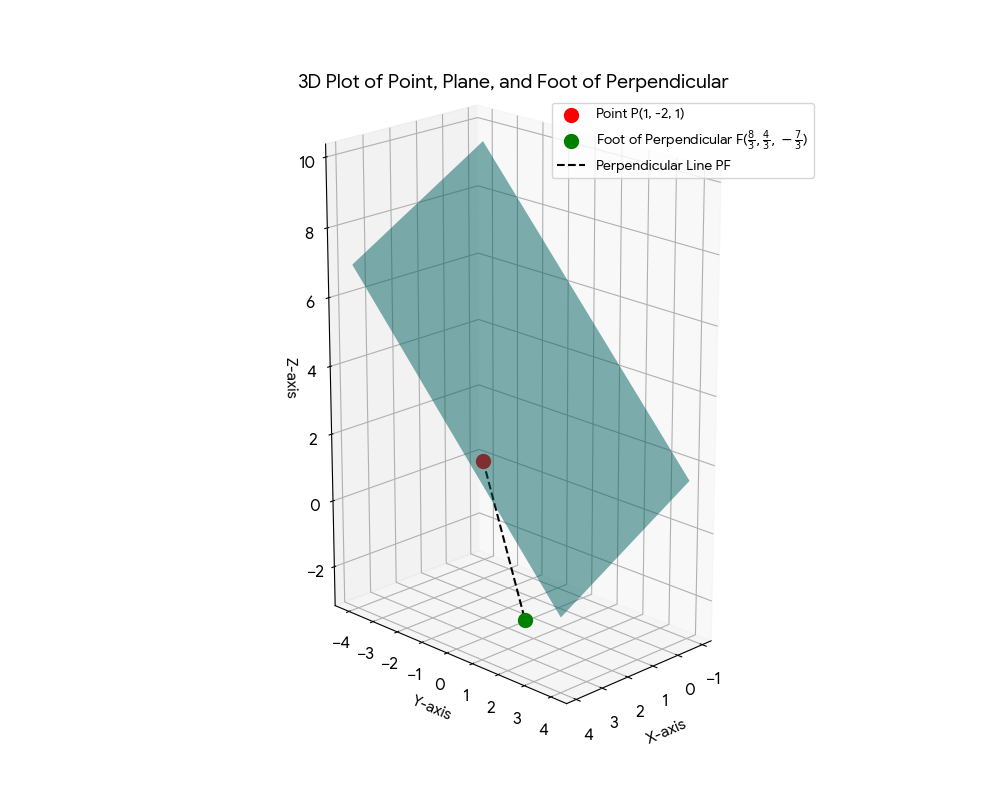
\includegraphics[width=\columnwidth]{figs/python_plot.png} 
\caption*{Plot of the curves}
\label*{Fig1}
\end{figure}


\end{document}
